\documentclass[conference]{IEEEtran}
% \usepackage{cite}
\usepackage{tikz, pgfplots}
\usepackage{amsmath,amssymb,amsfonts}
% \usepackage{algorithmic}
\usepackage{graphicx}
\usepackage{multirow}
% \usepackage{textcomp}
% \usepackage{xcolor}
\pgfplotsset{compat=1.18}
\graphicspath{{./images/}}
\def\BibTeX{{\rm B\kern-.05em{\sc i\kern-.025em b}\kern-.08em
    T\kern-.1667em\lower.7ex\hbox{E}\kern-.125emX}}

\begin{document}

\title{Evaluation of the Parameterized-Response Differential Evolution Trader-Agent}

\author{\IEEEauthorblockN{George Herbert}
\IEEEauthorblockA{\textit{Department of Computer Science} \\
\textit{University of Bristol}\\
Bristol, United Kingdom \\
cj19328@bristol.ac.uk}
}

\maketitle

\begin{abstract}
This paper reports results from market experiments containing Paramaterized-Response Differential Evolution (PRDE) trader-agents.
Each PRDE trader-agent in a market simultaneously uses differential evolution (DE) to adapt their own trading strategy to maximise profitability.
The DE algorithm within each PRDE trader is governed by two parameters: the differential weight coefficient $F$ and the number in population $\mathrm{NP}$.
Markets containing a homogeneous population of PRDE traders exhibit different dynamics depending on the values of $F$ and $\mathrm{NP}$
The first part of this paper evaluates the effect that these two parameters have on the dynamics of the market; while the latter part of this paper proposes an extension to the PRDE algorithm to further maximise profitability.
\end{abstract}

\begin{IEEEkeywords}
Automated Trading, Financial Markets, Adaptive Trader-Agents, Differential Evolution
\end{IEEEkeywords}

\section{Introduction}

Automated trading accounts for an unprecedented amount of activity in modern financial markets.
These algorithms have the ability to execute trades at a frequency simply unachievable for humans beings; thus, the behaviour of many of these markets has significantly shifted.
Notably, the `flash crash' in US financial markets on 6 May 2010 has been partially attributed to high-frequency trading algorithms aggressively reselling short-term positions to one another.
Modern automated trading algorithms have the additional quality of being adaptive: they adjust their strategy to extract maximum profit from the market in which they are operating.
These contemporary markets---in which competing adaptive algorithms are simultaneously engaged in coninual adjustment to maintain profitability---can be described as \textit{coevolutionary} systems.

Large amounts of research has been conducted to understand the dynamics of these markets.
Recently, Cliff introduced the \textit{Parameterized-Response Zero-Intelligence} (PRZI) \cite{PRZI} trader: a nonadaptive generalisation of Gode and Sunder's Zero-Intelligence Constrained (ZIC) \cite{GodeSunder} trader.
The difference lies in the probability mass function (PMF) used to generate quote prices.
Each individual ZIC trader samples their quote price from a fixed uniform distribution, whereas each PRZI trader is governed by a strategy parameter $s\in[-1, 1]\in\mathbb{R}$ that determines the PMF the trader samples from; the shape of this PMF determines how `urgent' or `relaxed' the trader acts.
As $s\to1$ the distribution is evermore biased towards `urgent' quote prices---those closest to the least profitable price for the trader, but most likely to attract a willing counterparty---conversely, as $s\to-1$, the distribution is biased towards `relaxed' quote prices---those that generate the most profit for the trader, but are considerably less likely to attract a counterparty.
When $s=0$, the PMF is uniform, identical to that of a ZIC trader.

\textit{PRZI Stochastic Hillclimber} (PRSH) \cite{PRSH} is an adaptive extension to the PRZI also introduced by Cliff.
The strategy parameter $s$ is dynamically altered by the algorithm in an attempt to increase profitability.
Each PRSH trader maintains a private local population $\mathcal{K}$ of $k$ strategy parameters; each of which it evaluates for a specific period of time via a loop to identify which is most profitable.
The most profitable strategy $s_0$ is `mutated' $k-1$ times; these $k$ values comprise the new elements of set $\mathcal{K}$.

\textit{PRZI Differential Evolution} (PRDE) \cite{PRDE} is further adaptive extension of the PRZI algorithm, and a successor to PRSH; it is the most recent algorithm published by Cliff in the PRZI `family' of trader-agents.
It replaces the simple stochastic hill-climber with a \textit{differential evolution} (DE) optimisation system \cite{StornPrice}.
Each PRDE trader maintains its own DE system with a population of candidate $s$-values of size $\mathrm{NP}\ge4$, which for trader $i$ can be denoted by $s_{i,1},s_{i,2},...,s_{i,\mathrm{NP}}$; the value $\mathrm{NP}$ is referred to as the \textit{number in population}.
Once a particular strategy $s_{i,x}$ has been evaluated, three other distinct $s$-value are chosen at random from the population maintained by trader $i$: $s_{i,a}$, $s_{i,b}$ and $s_{i,c}$ such that $x\ne a\ne b\ne c$.
A new candidate strategy $s_{i,y}$ is constructed as follows:
\[
s_{i,y}\leftarrow\max(\min(s_{i,a}+F_i(s_{i,b}-s_{i,c}),1), -1)
\]
where $F_i$ is the trader's \textit{differential weight} coefficient.
The fitness of $s_{i,y}$ is evaluated and if it performs better than $s_{i,x}$ then $s_{i,y}$ replaces $s_{i,x}$; otherwise, it is discarded and the next randomly selected strategy is evaluated.
This is very similar to the original description of the DE/rand/1 algorithm as described by Storn and Price \cite{StornPrice}, with a four key differences: $\max$ and $\min$ functions have been incorporated to constrain the output $s_{i,y}$ to the range $[-1,1]$; the conventional DE notion of crossover is not relevant because the behaviour of each PRZE trader is governed by only a single scalar value $s$; the DE algorithm in PRDE is a steady-state evolutionary algorithm as opposed to a generational evolutionary algorithm, which provides a small storage advantage; and Cliff introduced a simple vector-perbutation mechanism to deal with convergence issues that arised from $s_{i,b}-s_{i,c}$ tending very close to zero.
The vector-perbutation mechanism works as follows: if at any time the standard deviation of the candidate $s$-values in trader $i$'s private population is less than $0.0001$, then a randomly selected candidate is provided a value drawn at random from the uniform distribution $\mathcal{U}(-1,1)$.
This can be thought of a `mega-mutation' to the trader's set of $s$-values---a countermeasure to convergence.

Cliff's conducted experiments on the \textit{Bristol Stock Exchange} (BSE) (see \cite{BSE, BSEPaper}) to analyse the coevolutionary dynamics of markets populated entirely by PRSH and PRDE traders.
BSE is a freely-available, open-source simulation a LOB-based financial exchange.
Notably, Cliff identified that markets populated by PRDE traders were approximately 100\% more economically efficient than those populated by PRSH traders \cite{PRDE}.
However, the PRDE traders implemented in Cliff's experiments did not deviate from a differential weight of $F=0.8$ and a number in population of $\mathrm{NP}=4$ (i.e. the minimum viable value).
He stressed the importance of future work to explore the effects on the market's dynamics of altering these key parameters.
Cliff proposed two lines of future research.
He proposed an exploration into the effects on the market's dynamics of altering the two key parameters homogeneously---with all traders maintaining the same values of $F$ and $\mathrm{NP}$ in a given market session.
He also proposed an arguably more intriguing exploration into effects that arise from altering the two key parameters heterogeneously---with different traders being provided different values of $F$ and $\mathrm{NP}$.

\section{Homogeneous Exploration of $F$ and $\mathrm{NP}$}

\subsection{Overview of the Combined Effect of $F$ and $\mathrm{NP}$}

My initial experiments in this paper focus on the combined effect that $F$ and $\mathrm{NP}$ have on the dynamic of a coevolutionary market.
I designed a set of experiments with a similar setup as Cliff in \cite{PRDE} in which BSE was used to simulate a financial market for a single abstract tradeable commodity.
In each market simulation, I implemented a homogeneous population of $N_T=30$ PRDE traders with an equal number of buyers $N_B$ and sellers $N_S$ (i.e. $N_B=N_S=15$).
The population in a given experiment was homogeneous with respect to the fact that all PRDE traders had the same differential weight $F$ and the same number in population $\mathrm{NP}$.
Each simulation had what economists refer to as perfect elasticity of supply and demand: all $N_B$ buyers were provided a limit price of $\lambda_B=\$140$ per unit, whilst all $N_S$ sellers were provided a limit price of $\lambda_S=\$60$ per unit.
This produced a market in which every active trader could, in theory, find a willing counterparty to trade with.
In the simulation, after two traders engaged in a trade, they were rendered inactive until their stock was replenished, which occurred approximately every five seconds.
I ran each experiment for 100 simulated days on an Apple MacBook Pro with the M1 Pro chip, which took approximately three hours running at 800x real-time.

In market simulations such as these, `profit' is conventionally used to refer to the absolute difference between the trader's limit price and the transaction price.
Figure \ref{profit_grid} displays a heatmap showing the combined profit extracted from the market by the population of $N_B$ buyers and $N_S$ sellers.
Considering each experiment used an identical quantity of traders and identical limit prices, the total profit extracted is indicative of market efficiency.
As such, there is a clear association between the configuration of $F$ and $\mathrm{NP}$ and the efficiency of the market.
However, the cause of this association is not obvious from inspecting the raw values.

\begin{figure}[htbp]
    \centerline{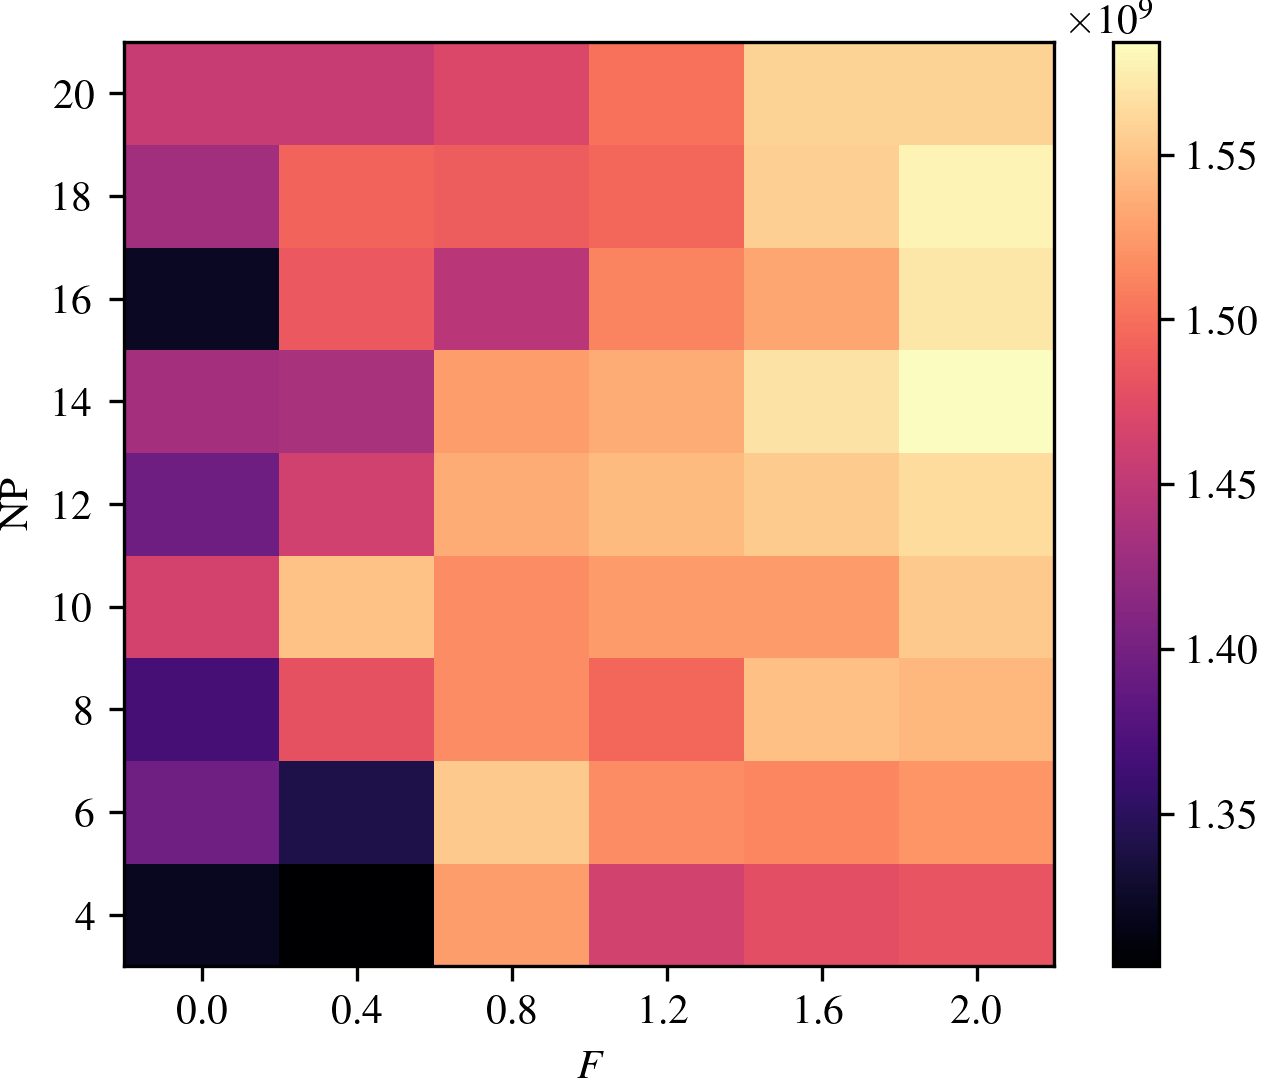
\includegraphics[width=\columnwidth]{profit_grid.png}}
    \caption{
        Relationship between the differential weight coefficient $F$, the number in population $\mathrm{NP}$ and the total profit extracted by all PRDE traders in the market.
        Horizontal axis is the differential weight coefficient $F$; vertical axis is the number in population $\mathrm{NP}$.
        The intensity of pixel shading represents the total profit extracted from the market during a given 100-day simulation.
        See text for further discussion.
    }
    \label{profit_grid}
\end{figure}

To further understand this association, one must consider how the $s$-value of a given PRDE trader at a particular point in time affects the probability of it finding a counterparty to trade with.
For a given trader, as $s\to1$ (i.e. increasingly `urgent') the trader's quote prices are evermore likely to attract a counterparty; the reverse is true as $s\to-1$ (i.e. increasingly `relaxed').
As such, there is a strong relationship between the amount of time the traders in the market are `urgent' and the quantity of trades in the market session.
Due to each experiment having perfect elasticity of supply and demand, for a given trade at price $P$, the seller's profit can be denoted $P-\lambda_S$, whilst the buyer's profit can be denoted $\lambda_B-P$.
Therfore, the combined profit is as follows:
\[
  (P-\lambda_S) + (\lambda_B-P)=\lambda_B-\lambda_S
\]
In other words, the profit extracted from the market from any given trade is constant.
As such, the total profit extracted from the entirety of a given 100-day market session is directly proportional to the number of trades, which, as mentioned, is related to the amount of time traders in the market are `urgent'.
I proved experimentally that this relationship indeed manifests, as evident in Figure \ref{strategy_profit}.
There was a strong positive correlation between the total amount of time the traders in the market spent with $s>0.5$ (i.e. `very urgent') and the total profit extracted from the market.
In fact, the coefficient of determination of the relationship is $R^2=0.72$; thus, a large amount of the variance in the profit extracted from the market can be explained by this relationship.
Considering the inherent stochasticity in market simulations, this can be considered a strong relationship.

\begin{figure}[htbp]
    \centerline{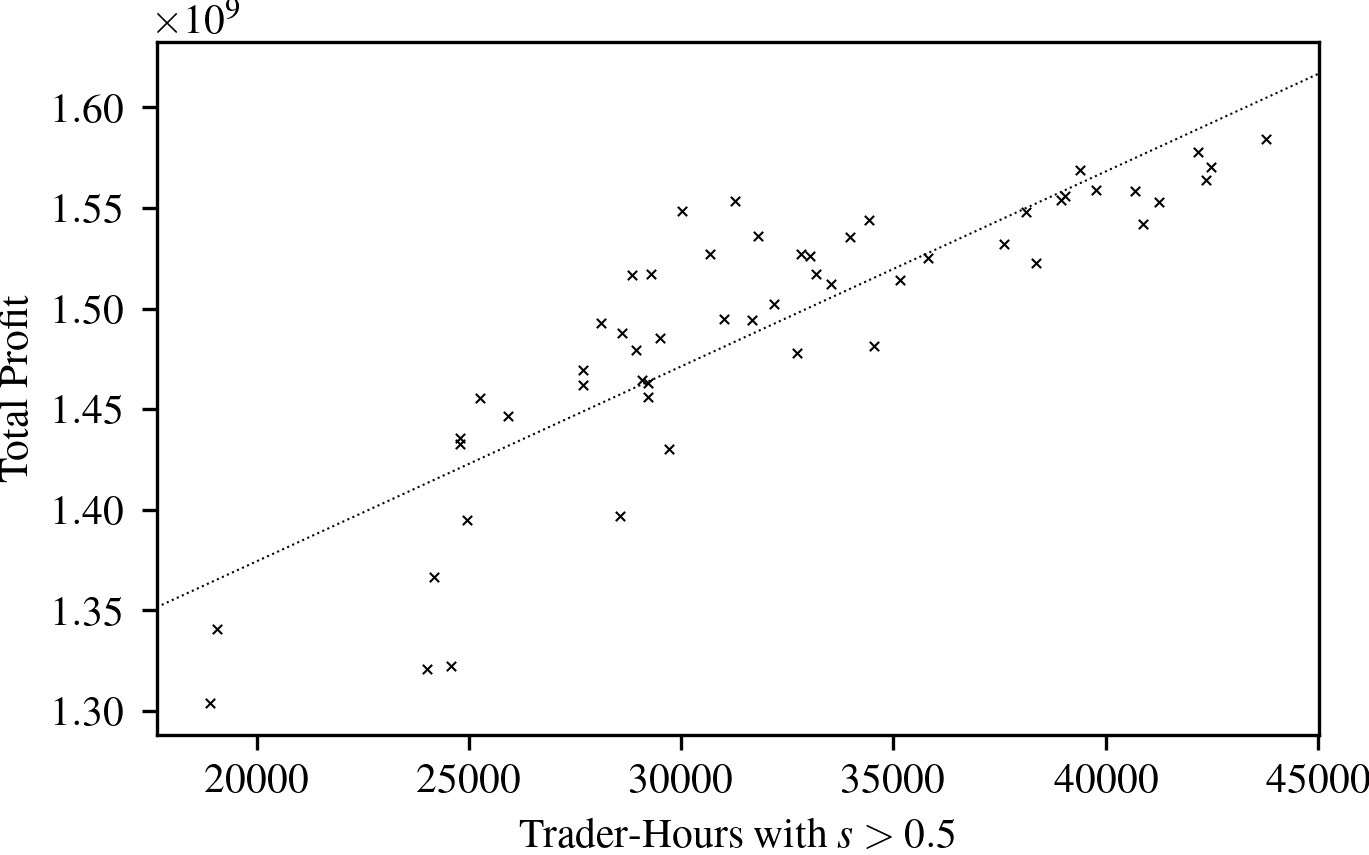
\includegraphics[width=\columnwidth]{strategy_profit.png}}
    \caption{
        Relationship between the number of trader-hours in the market playing `very urgent' stratgies (i.e. $s>0.5$) and the total profit extracted by all traders in the market.
        Horizontal axis is the number of trader-hours where $s>0.5$; vertical axis is the total profit extracted from the market during a given 100-day simulation.
        The line shows linear regression; $R^2=0.72$.
        See text for further discussion.
    }
    \label{strategy_profit}
\end{figure}

Due to this relationship, if every trader was aware of the perfect elasticity of supply and demand, and decided to act in the best interests of the market, they would behave like a PRZI trader with $s=1$.
This would maximise the number of trades in the market, and thus maximise the profit extracted from the market.
However, each trader is only aware of their own limit price, and additionally only seeks to optimise their own profitability.
It is this that introduces inherent inefficiency into the market.

\subsection{Analysis of the Effect of $F$}

As mentioned, much of the variance in the efficiency of the market can be explained by the quantity of `very urgent' traders residing in it.
To this end, the influence that $F$ has on the total profitability can be primarily attributed to how it influences the `urgency' of the traders.
This was confirmed using data from the market simulations, which showed that larger values of $F$ tended to increase the traders' `urgency'.
This is evident in Figure \ref{F_strats}, which shows that 77\% of the variance in the number of trader-hours spent with $s>0.5$ can be explained purely the differential weight of the PRDE traders.

\begin{figure}[htbp]
    \centerline{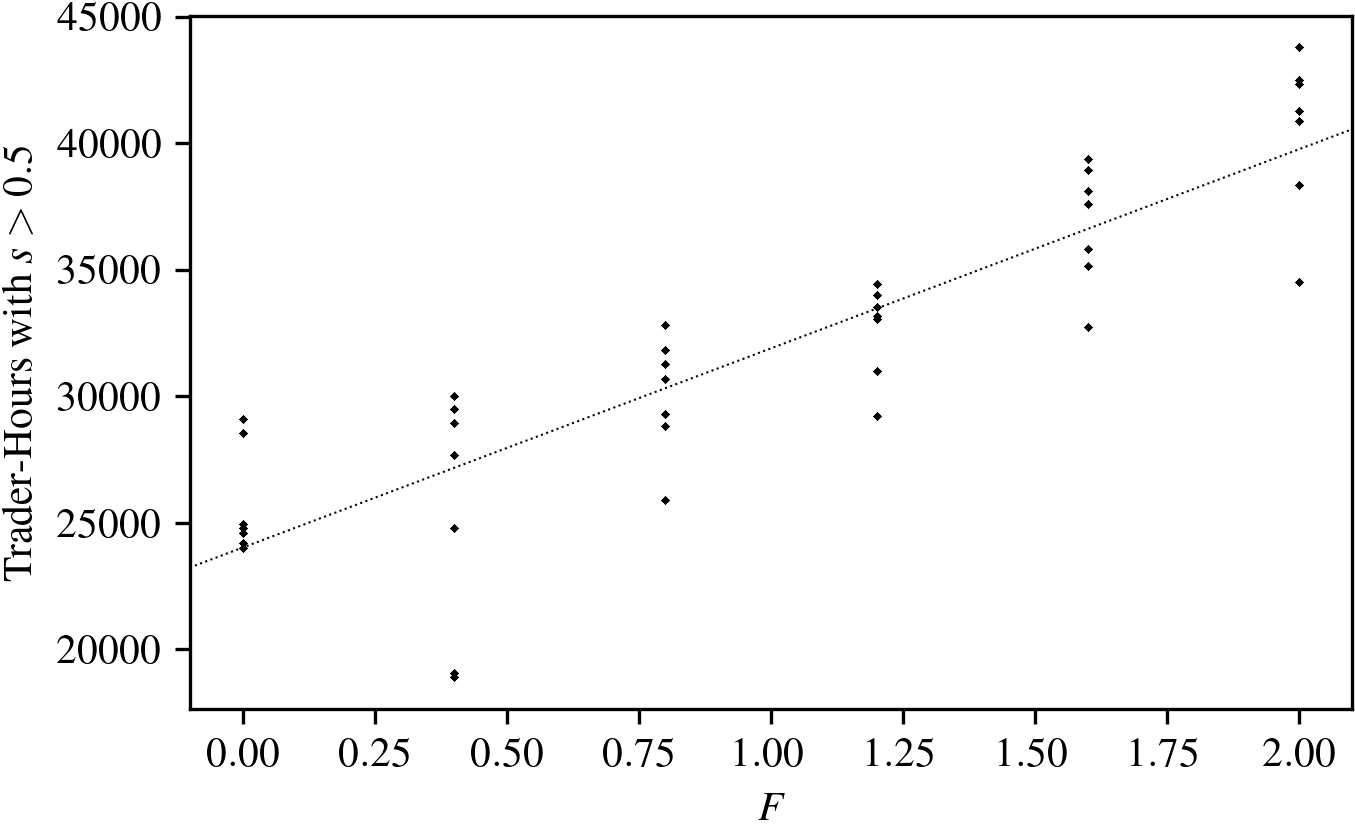
\includegraphics[width=\columnwidth]{F_strats.png}}
    \caption{
        Relationship between $F$ and the number of trader-hours in the market playing `very urgent' strategies (i.e. $s>0.5$).
        Horizontal axis is the differential weight coefficient $F$; vertical axis is the number of trader-hours where $s>0.5$.
        The line shows linear regression; $R^2=0.77$.
        See text for further discussion.
    }
    \label{F_strats}
\end{figure}

Figure \ref{k=14_strats} shows how the `urgency' of the PRDE traders develops over the 100-day market sessions for different values of $F$.
It displays the percentage of traders playing with $s>0.5$ throughout multiple market sessions when $\mathrm{NP}=14$.
The graph highlights that the proportion of `urgent' strategies increased significantly faster for larger values of $F$.
For example, when $F=0.4$, it took approximately 90 days for the seven-day simple moving average to increase to it's maximum percentage of 37.5\%.
This is a large amount of time considering even a uniform distribution of $s$-values would be expected to achieve 25\%.
Conversely, when $F=2$, the moving average had reached this percentage after only seven days.

\begin{figure}[htbp]
    \centerline{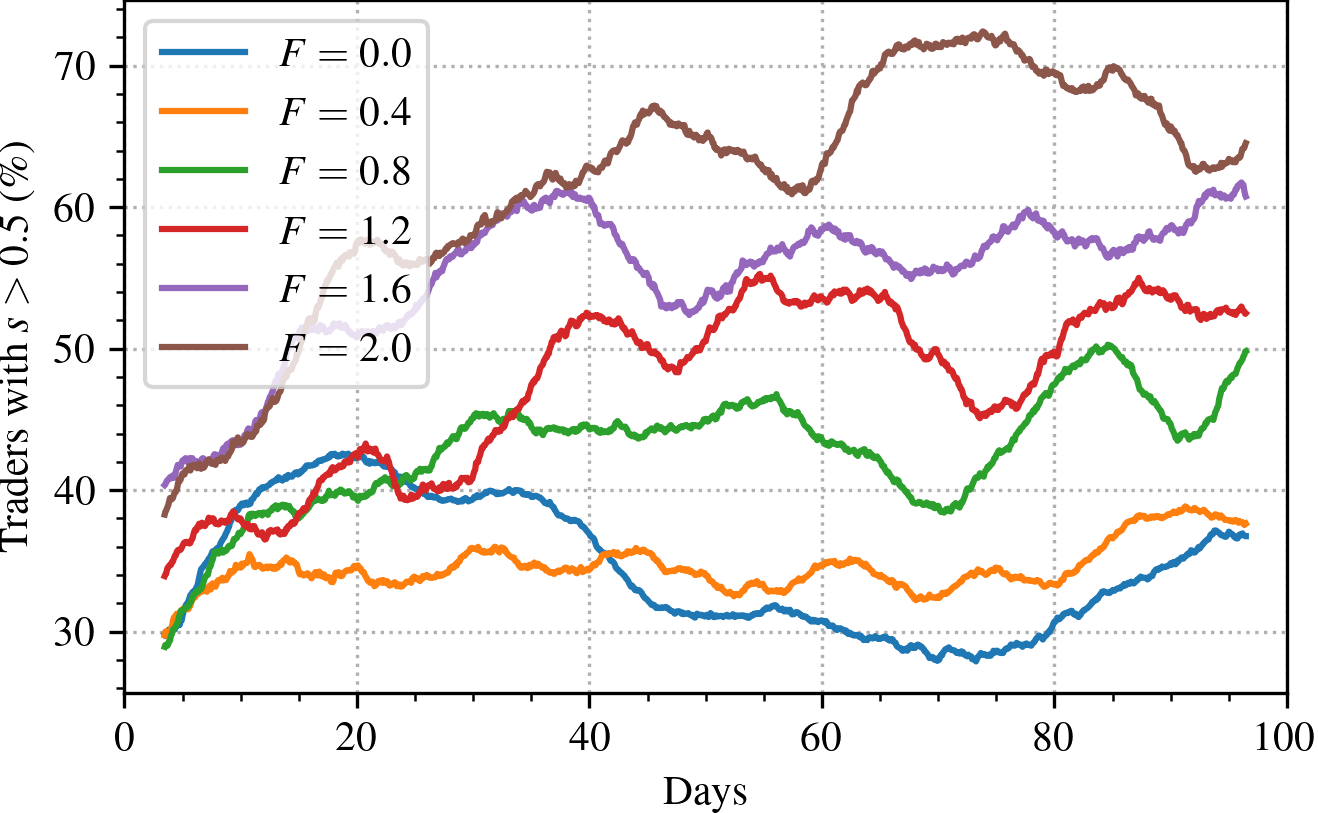
\includegraphics[width=\columnwidth]{k=14_strats.png}}
    \caption{
        Plot of the percentage of `very urgent' traders from multiple 100-day experiments in a market populated entirely by PRDE traders with $\mathrm{NP}=14$.
        Horizontal axis is time, measured in days; vertical axis is the proportion of traders with an $s$-value of $s>0.5$.
        Each line is a seven-day simple moving average of the proportion for different values of $F$.
        See text for further discussion.
    }
    \label{k=14_strats}
\end{figure}

The reason for this effect can be explained mathematically.
Taking the extreme example of $F=0$, the equation to derive a new candidate stratety $s_{i,y}$ to replace $s_{i,x}$ simply becomes $s_{i,y}\leftarrow s_{i,a}$.
Therefore, for a given trader $i$, following the evaluation period of $s_{i,y}$, the value of $s_{i,x}$ can either remain the same, or take on the value of $s_{i,y}=s_{i,a}$, in which case two or more of the $s$-values in the local population will be identical---the `genetic diversity' will be reduced.
In fact, the only time a new $s$-value can be introduced into trader $i$'s local population is when the diversity of $s$-values becomes so constrained a `mega-mutation' occurs, in which case a new $s$-value is sampled from $\mathcal{U}(-1,1)$.
As a result, the distribution of $s$-values in the entire population of PRDE traders struggles to deviate significantly from uniformity throughout the entirety of the 100-day market session.
This ultimately produces a market containing a wide range of both `urgent' and `relaxed' buyers and sellers, which is inefficient since many of the more `relaxed' traders will be unable to find a willing counterparty.
An example of such a distribution of $s$-values can be seen in Figure \ref{k=14,F=0.0_buy_strats}, which displays a heatmap of individual strategy values for the proportion of 15 PRDE buyers when $F=0$ and $\mathrm{NP}=14$.
While the case of $F=0$ is extreme, I found experimentally that the market increasingly exhibits the inefficient dynamics described here as $F$ tends towards $0$.

\begin{figure}[htbp]
    \centerline{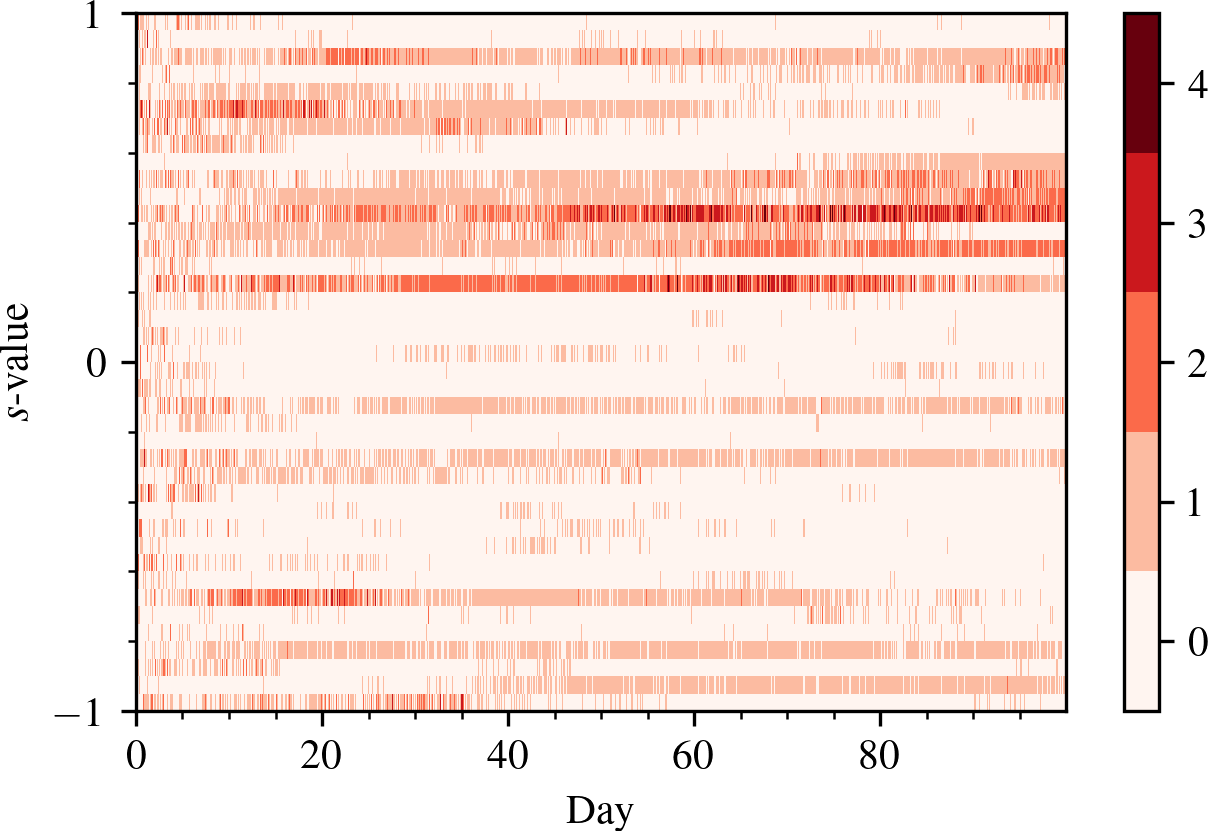
\includegraphics[width=\columnwidth]{k=14,F=0.0_buy_strats.png}}
    \caption{
        Heatmap of individual strategy-values for the population of 15 PRDE buyers in a market populated entirely by PRDE traders with $F=0$ and $\mathrm{NP}=14$.
        Horizontal axis is time, measured in days; vertial axis is the strategy value pixelated into 40 bins of size 0.05.
        The intensity of pixel shading increases with the number of PRDE sellers in the population currently trading with a strategy value in a given 0.05 range.
        See text for further discussion.
    }
    \label{k=14,F=0.0_buy_strats}
\end{figure}

On the other extreme of the spectrum when $F=2$, a very different market dynamic tends to manifest.
This is evident in Figure \ref{k=14,F=2.0_buy_strats}, which displays a heatmap for the 15 PRDE buyers whereby $F=2$ and $\mathrm{NP}=14$.
Unlike the more uniform distribution of $s$-values exhibited when $F=0$, the $s$-values in Figure \ref{k=14,F=2.0_buy_strats} were bimodal at the two extremes of $s\approx-1$ and $s\approx1$, with the peak at $s=1$ being slightly larger.
Moreso, both the buyers and sellers displayed this behaviour.
Again, this can be explained mathematically using the equation to derive a new candidate stratety $s_{i,y}$ to replace $s_{i,x}$.
The value of trader $i$'s differential coefficient $F_i$ is directly proportional to $F_i(s_{i,b}-s_{i,c})$.
Thus, assuming $s_{i,b}-s_{i,c}$ is non-zero, the value of $s_{i,y}$ is more likely to be $-1$ or $1$ as $F_i$ increases.
This creates a market dynamic in which there is very quickly a number of of both extremely `urgent' and extremely `relaxed' buyers and sellers.
This large number of urgent traders that exist throughout the market session enable a large amount of profit to be extracted from the market.
Furthermore, I found experimentally that for larger values of $F$, this bimodal behaviour is evermore prominant.

\begin{figure}[htbp]
    \centerline{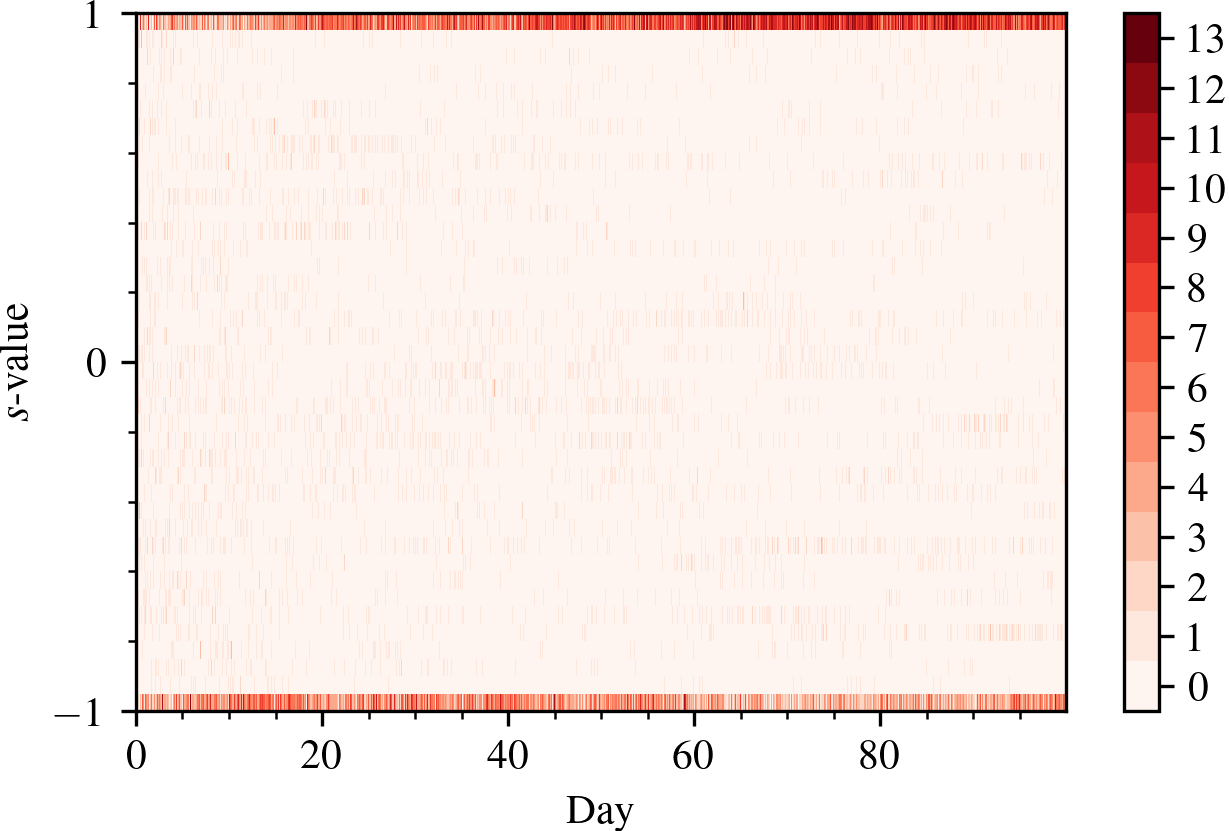
\includegraphics[width=\columnwidth]{k=14,F=2.0_buy_strats.png}}
    \caption{
        Heatmap of individual stratey values for the population of 15 PRDE buyers in a market populated entirely by PRDE traders with $F=2$ and $\mathrm{NP}=14$.
        Format is the same as for Figure \ref{k=14,F=0.0_buy_strats}.
        See text for further discussion.
    }
    \label{k=14,F=2.0_buy_strats}
\end{figure}

\subsection{Analaysis of the Effect of $\mathrm{NP}$}

The effect that the number in population $\mathrm{NP}$ has on the efficiency of a coevolutionary market is more complex. 
For smaller values of $F$, the influence of $\mathrm{NP}$ is significantly noisy, as is evident in Figure \ref{profit_grid}.
However, for larger values of $F$, there is a more clear, causal relationship.
As mentioned, the `urgency' of the traders in the market is indicative of the market's efficiency.
In the simulations I conducted, the relationship between $\mathrm{NP}$ and this `urgency' was approximately quadratic, especially for larger values of $F$.
This is evident in Figure \ref{F=2.0_strats}, which displays this relationship for the simulations in which $F=2$.

\begin{figure}[htbp]
    \centerline{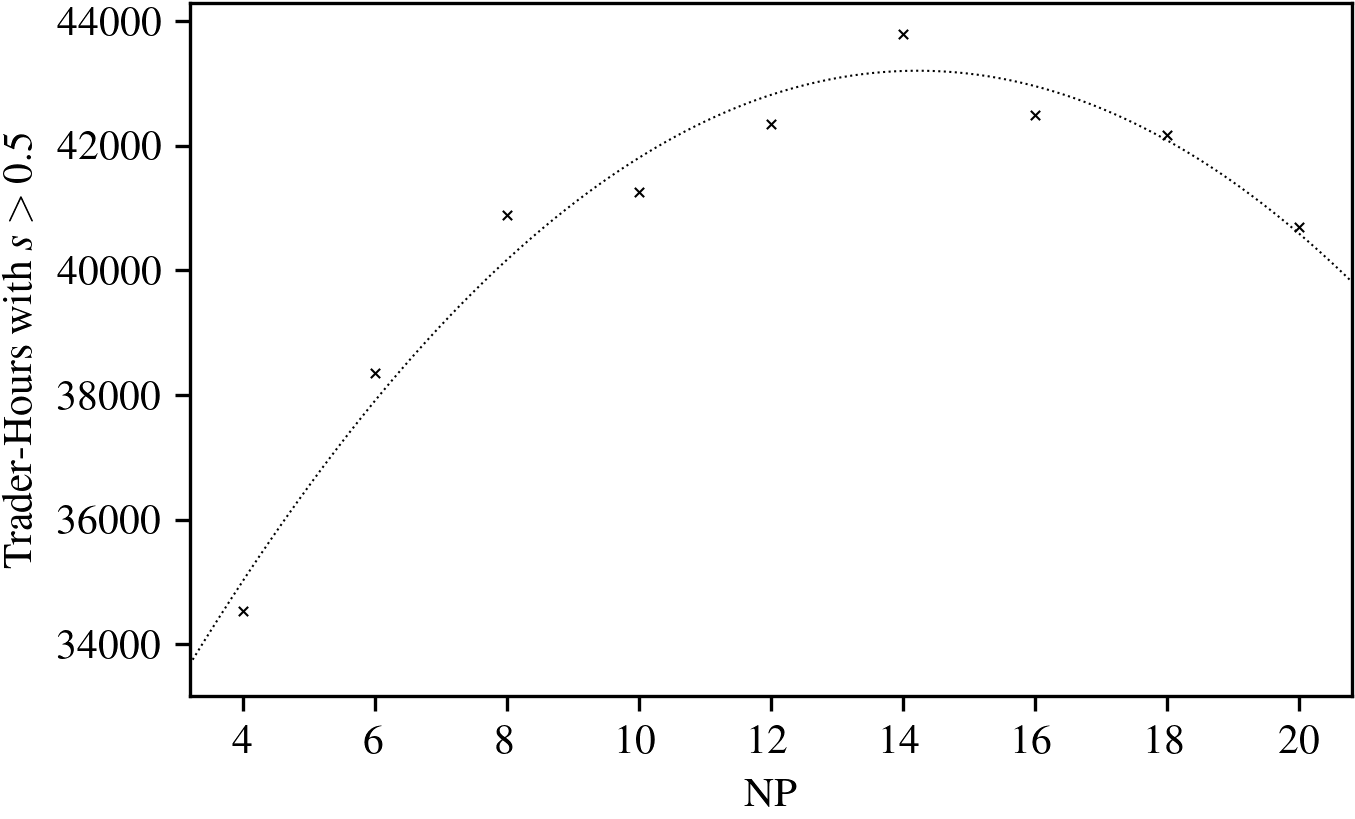
\includegraphics[width=\columnwidth]{f=2.0_strats.png}}
    \caption{
        Relationship between $\mathrm{NP}$ and the number of trader-hours in the market playing `very urgent' strategies (i.e. $s>0.5$) when $F=2.0$.
        Horizontal axis is the number in population $\mathrm{NP}$; vertical axis is the number of trader-hours where $s>0.5$.
        The line shows quadratic regression; $R^2=0.96$.
        See text for further discussion.
    }
    \label{F=2.0_strats}
\end{figure}

This quadratic relationship can be explained as the combined effect that $\mathrm{NP}$ has on the number of very `urgent' traders in the market, and the time it takes the traders in the market to improve on the initial random conditions.
As mentioned, larger values of $F$ induce a bimodal distribution of $s$-values at $s\approx -1$ and $s\approx 1$.
Using $\mathrm{NP}=\mathrm{4}$ as an example, an individual trader can have at most three $s$-values of $s\approx 1$, because as soon as the fourth $s$-value becomes 1, a `mega-mutation' occurs.
Conversely, when $\mathrm{NP}$ is larger, individual traders are able to accumulate a larger proportion of $s$-values of $s\approx 1$ in their private populations.
This means that homogeneous populations of PRDE traders with larger values of $\mathrm{NP}$ produce a market dynamic with more `very urgent' traders, which produces a more efficient market.
However, this trend is not linear because for especially large values of $\mathrm{NP}$, an inverse relationship between $\mathrm{NP}$ and the number of `very urgent' traders in the market manifests.
This is because, for a given PRDE trader, the probability than an $s$-value in the trader's private population is selected to be evaluated next is $\mathrm{NP}^{-1}$.
In other words, it is inversely proportional to $\mathrm{NP}$.
Therefore, in homogeneous populations of PRDE traders with larger values of $\mathrm{NP}$, it takes significantly longer to iteratively improve on the initial random conditions in the entire local population of $s$-values.
As a result, it takes significantly longer for the PRDE traders to accumulate a large number of $s$-values of $s>0.5$, and as such the market is less efficient.

\section{Heterogeneous Exploration of $F$ and $\mathrm{NP}$}

The experiments conducted to this point all involved homogeneous populations of PRDE traders.
The results clearly showed that the markets containing PRDE traders with large values of $F$ and moderately large values of $\mathrm{NP}$, such as $F=2$ and $\mathrm{NP}=14$, managed to extract the most profit from the market.
This was simply because these combinations of $F$ and $\mathrm{NP}$ influenced the DE algorithm to sustain more highly `urgent' $s$-values.
However, contemporary real-world markets are not comprised of homogeneous populations of automated trading-agents; real-world markets contain a multitude of different trading algorithms, all using different adaptive algorithms to maximise profitability, as well as a number of human traders.
Thus, I sought to investigate whether the profitability of a given combination of $(F, \mathrm{NP})$ in a homogeneous market was correlated to the profitability of the same combination in a heterogeneous market.
To do so, I ran a follow-up experiment with a very similar setup to that described previously to control for extraneous variables.
I similarly used BSE to simulate a financial market with $N_T=30$ PRDE traders with an equal number of buyers $N_B$ and sellers $N_S$ (i.e. $N_B=N_S=15$).
I used a limit price of \$140 per unit for the $N_B$ buyers and \$60 per unit for the $N_S$ sellers, and ran the experiment for 100 simulated days.
In fact, the only difference was the fact that I populated the market with heterogeneous PRDE traders rather than homogeneous PRDE traders.
I supplied each of the $N_B$ buyers and $N_S$ sellers an $(F,\mathrm{NP})$ combination from the 15 elements in the following set:
\[
  \left\{ (F, \mathrm{NP}) \mid F\in\{0, 0.4, 0.8, 1.6, 2\} \land \mathrm{NP} \in \{4, 12, 20 \} \right\}
\]
such that each buyer had a corresponding seller with the same element, but no two buyers or sellers had the same combination.

The total profit extracted from the heterogeneous market---which is indicative of market efficiency---was comfortably within the range of the homogeneous experiments at approximately 1.43 billion.
In fact, it was within 1\% of the mean profit extracted from the homogeneous experiments in which the $(F,\mathrm{NP})$ combinations comprised the heterogeneous experiment.
However, interestingly, there was no discernible relationship between the profitability of a trader with a given $(F, \mathrm{NP})$ combination in the homogeneous experiments and the same $(F, \mathrm{NP})$ in the heterogeneous experiment, as evident in Figure \ref{heterogeneous_homogeneous}.

\begin{figure}[htbp]
    \centerline{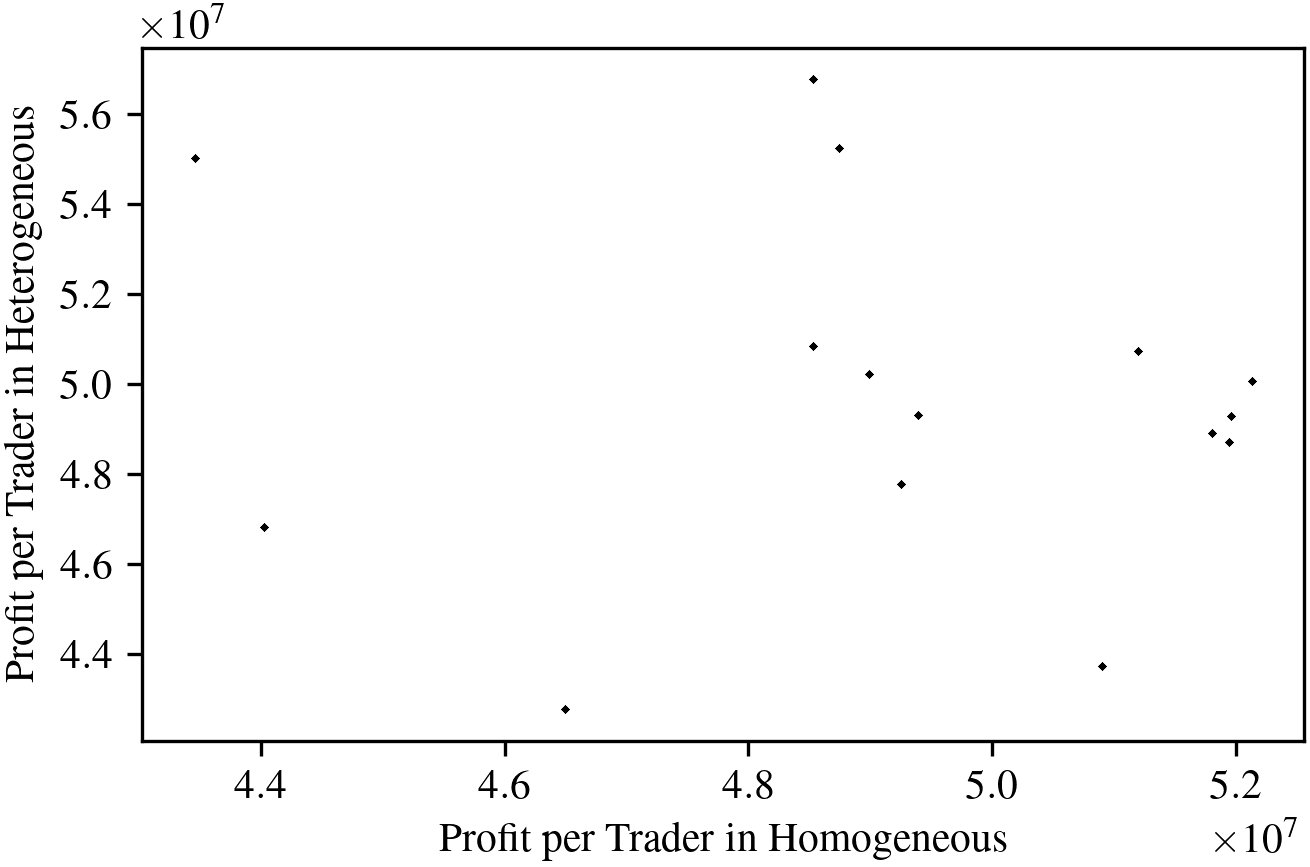
\includegraphics[width=\columnwidth]{heterogeneous_homogeneous_scatter.png}}
    \caption{
        Relationship between the profitability per trader in the homogeneous experiments and the heterogeneous experiments.
        Horizontal axis is the mean profit per trader in a given homogeneous experiment for a specific combination of $F$ and $\mathrm{NP}$; vertical axis is the mean profit per trader in the heterogeneous experiment for the same combination of $F$ and $\mathrm{NP}$.
        See text for further discussion.
    }
    \label{heterogeneous_homogeneous}
\end{figure}

This indicates that the effect of $F$ and $\mathrm{NP}$ differs according to the population of traders in the market.
In effect, there is no absolute `optimal' combination that will consistently extract the maximum profit, because the behaviour of the other traders in the market strongly influences the control that $F$ and $\mathrm{NP}$ have.

\section{Extending PRDE}

\subsection{Motivation}

The experiments showed that the behaviour of the PRDE traders was highly influenced by the differential weight coefficient $F$ and the number in population $\mathrm{NP}$.
Moreso, it was evident that no one combination was consistently most profitable---the profitability was highly dependent on the other traders in the market, as well as the type of market.
As such, I hypothesised that a trader similar to PRDE, that automatically controlled the value of $F$ would be far more profitable across a variety of different markets.

\subsection{JADE}

JADE \cite{ZhangSanderson} is a DE algorithm that automatically updates the control parameter $F$ to appropriate values, and therefore removes the requirement for a user to have prior knowledge about the relationship between $F$ and the characteristics of the optimisation problem.
In light of this, I replaced the DE/rand/1 variant in PRDE with a variant of the JADE algorithm to produce a new trader agent: \textit{Parameterized-Response JADE} (PRJADE).
I hypothesised that PRJADE would provide better performance across a range of different markets, since the user would not require prior knowledge of the market dynamic.

To implement JADE in PRJADE, I implemented a variant of the DE/Current-to-$p$-best/1 with archive mutation strategy \cite{ZhangSanderson}.
Each PRJADE trader maintains its own JADE system with a population of candidate $s$-values of size $\mathrm{NP}\ge 4$, which for trader $i$ in generation $g$ can be denoted by 
\[
    P=\{s_{i,g,1}, s_{i,g,2},...,s_{i,g,\mathrm{NP}}\}
\]
Once a particular strategy $s_{i,g,x}$ has been evaluated, three other distinct $s$-values are chosen: $s^p_{i,g,\text{best}}$ is randomly chosen as one of the top $p\%$ individuals in the population $P$; $s_{i,g,r_1}$ is randomly chosen from the population $P$ such that $s_{i,g,r_1}\ne s^p_{i,g,\text{best}}$; and $\tilde{s}_{i,g,r_2}$ is randomly chosen from $P\cup A$ such that $\tilde{s}_{i,g,r_2}\ne s_{i,g,r_1}\ne s^p_{i,g,\text{best}}$.
$A$ is an `archive' set of $s$-values: those $s$-values that previously failed in the selection process.

The mutation $s$-value in PRJADE is computed as follows:
\[
    \hat{s}_{i,g,x}=s_{i,g,x}+F_i\left(s^p_{i,g,\text{best}} - s_{i,g,x}\right) + F_i\left(s_{i,g,r_1} - \tilde{s}_{i,g,r_2}\right)
\]
The fitness of $\hat{s}_{i,g,x}$ is evaluated and if it performs better than $s_{i,g,x}$ then $\hat{s}_{i,g,x}$ replaces $s_{i,g,x}$ in generation $g+1$ (i.e. $s_{i,g+1,x}\leftarrow\hat{s}_{i,g,x}$); otherwise, it is discarded and the next strategy in the sequence $s_{i,g,x+1}$ is evaluated.

\subsection{Results}

\section{Conclusion}

\bibliographystyle{IEEEtran}
\bibliography{refs}

\end{document}
